\section{Vista Lógica} \label{vistaLogica}
A continuación se muestran 2 diagramas que describen, de manera estática, la estructura del sistema y su interacción con entidades externas.

\subsection{Diagrama Conceptual (Modelo de Dominio)}
Este diagrama muestra la interacción de eFuel con sistemas y agentes externos.

\begin{figure}[H]
    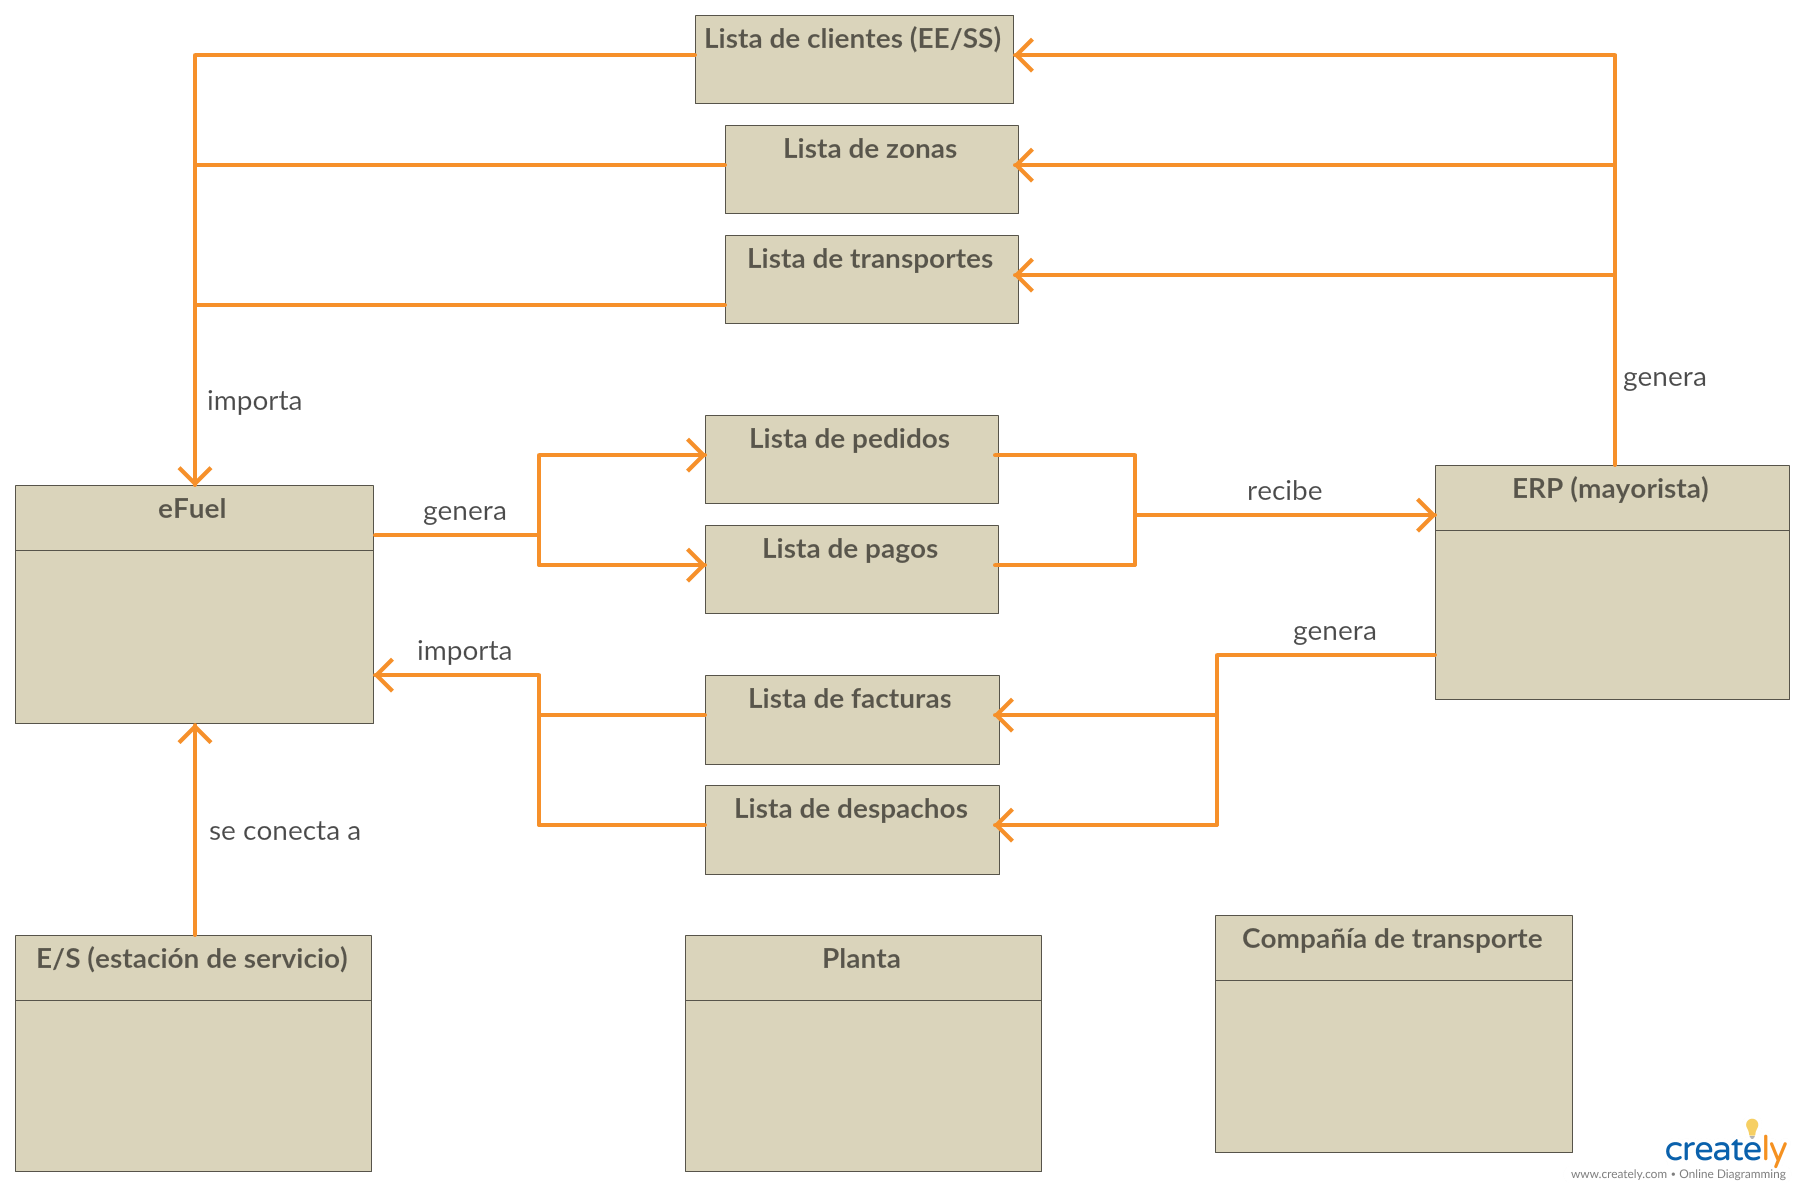
\includegraphics[width=\textwidth]{domain_model.png}
    \caption{Modelo de Dominio}
    \label{fig:domain_model}
    \centering
\end{figure}

\subsection{Diagrama de Clases}
A continuación se muestra un diagrama donde están representadas las principales entidades del sistema y las relaciones entre ellas. Las tablas con los bordes punteados son Doctypes de Umbraco representados como clases y los de linea continua son las clases principales del sistema (no son Doctypes de Umbraco).

\begin{figure}[H]
    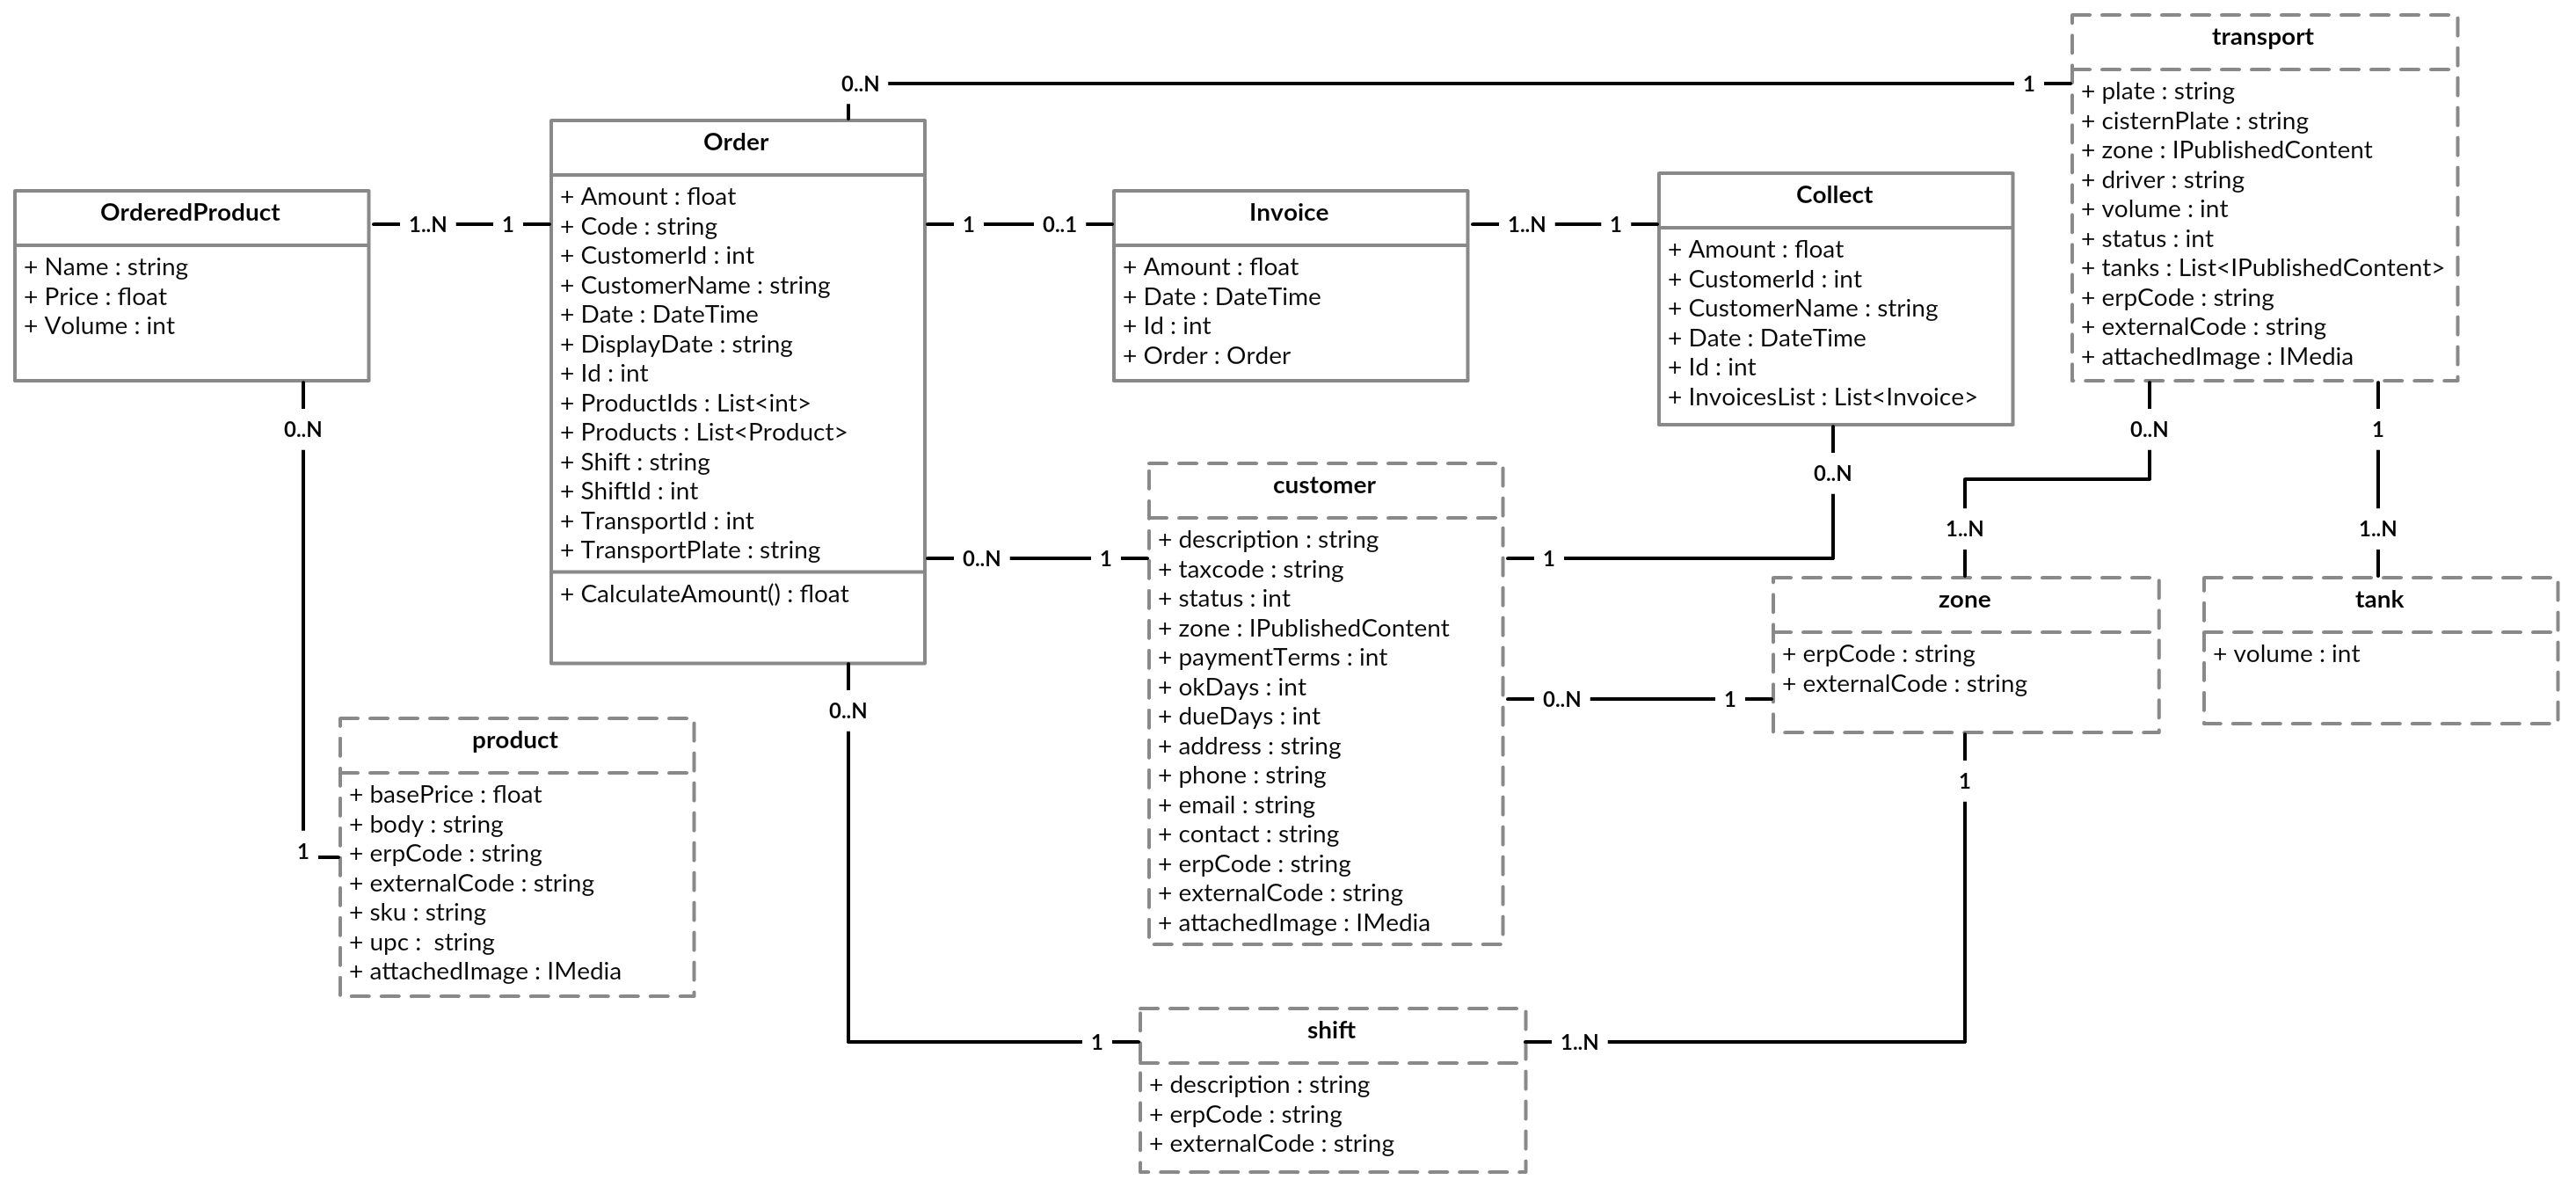
\includegraphics[width=\textwidth]{class_diagram.png}
    \caption{Diagrama de Clases de las entidades principales}
    \label{fig:class_diagram_main}
    \centering
\end{figure}